\subsection{Architettura del FrontEnd}

Come già specificato in precedenza nel Frontend è stato utilizzato, appunto, il pattern architetturale MVVM, ossia: quando l’utente esegue un’operazione nella WebApp (per esempio effettua una ricerca di un locale tramite il suo nome), il View-Model chiede al Model di scaricare i dati e/o effettuare le operazioni e rimane in attesa della risposta (nel caso di chiamate sincrone) oppure aspetta degli aggiornamenti e "osserva" (in caso di chiamate asincrone). Il Model invoca una API (che può essere una GET o una POST), la quale si interfaccerà con il Backend e, in caso di esito positivo, ritornerà la risposta o salverà i dati (in base all'operazione effettuata). \\
Una volta che il Model avrà finito l'operazione, ritornerà direttamente la risposta al View-Model, nei casi in cui è necessaria, oppure notificherà il View-Model che i dati "osservati" sono cambiati, il quale, allora, chiederà al Model di restituirgli i dati aggiornati. Successivamente, quando anche i dati del View-Model sono stati aggiornati, anche la View riceverà una notifica, stavolta dal View-Model, che gli chiederà di re-renderizzarsi con i nuovi dati, disponibili tramite il data-binding. 



\begin{figure}[H]
    \centering
    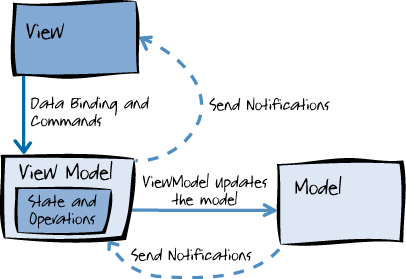
\includegraphics[scale=0.5]{Contenuto/Immagini/MVVM.png}
    \caption{Schema MVVM}
\end{figure}

In questo modo si ha una netta separazione tra chi salva ed elabora i dati (il Model) e chi li mostra (la View), mentre il View-Model funge da tramite tra le due parti. 
In accordo con il proponente, per realizzare la parte Frontend della WebApp, abbiamo scelto di utilizzare la libreria JavaScript React. Per l'aggiornamento dei dati nel Model e la notifica dei cambiamenti a questi al View-Model è stata utilizzata la libreria \textit{MobX}. Questa ci ha permesso di implementare il meccanismo degli Observer su React. 
Invece per la notifica alla View da parte del View-Model è stata utilizzata la libreria \textit{MobX-React} : questa permette di notificare la View e gli chiede di re-renderizzarsi, mostrando così i dati aggiornati (disponibili per il data-binding con il View-Model).



